\def\notedate{2022.03.09}
\def\currentauthor{Тришин И.В. (РК6)}

\notestatement{rndhpcblo}{Текущее представление графовых моделей в библиотеке comsdk}

На рисунке~\ref{fig:oldGraphStructure} представлена \textsf{UML}-диаграмма классов, связанных с представлением в \textsf{comsdk} ориентированного графа, описывающего организацию вычислительных процессов.

\begin{figure}[H]
    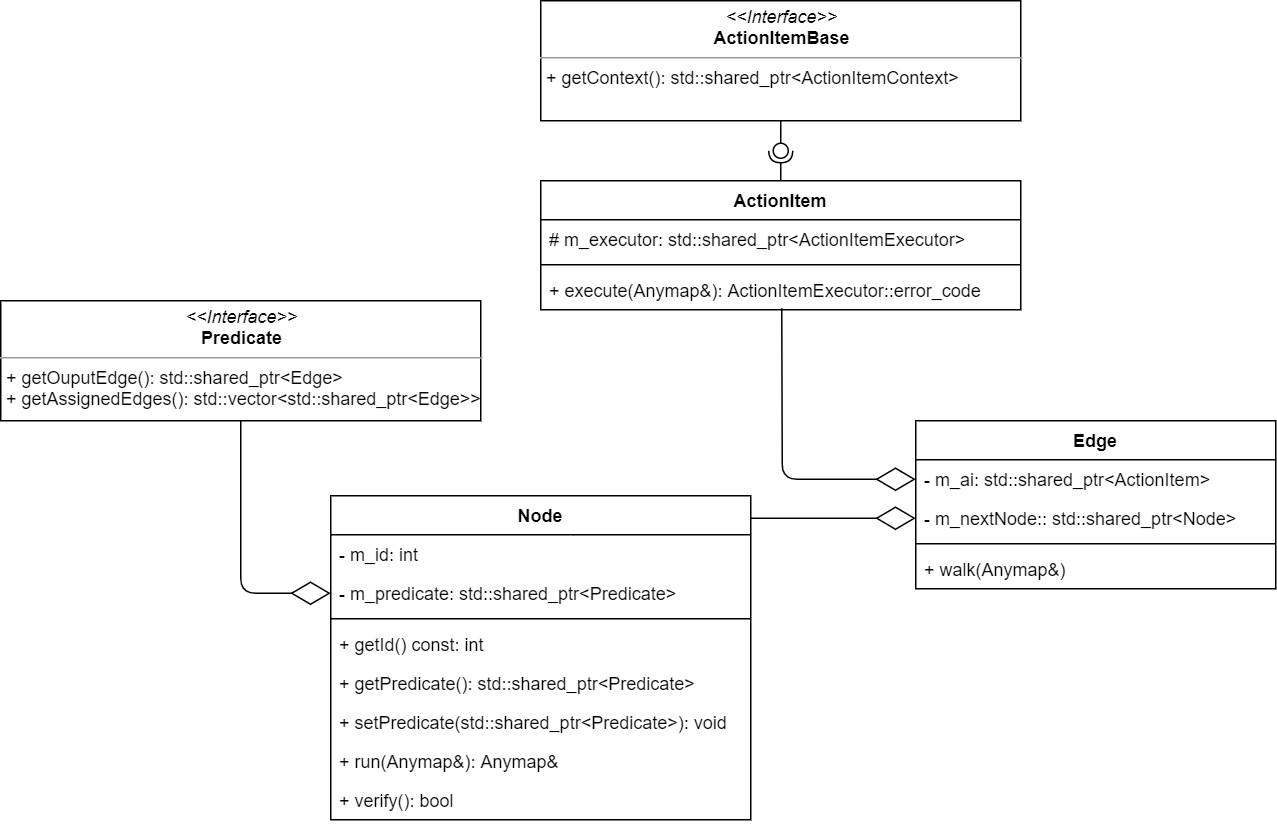
\includegraphics[width=\textwidth]{ResearchNotes/rndhpc_not_blo_2022_03_09/structure.png}
    \caption{Текущая структура классов, связанная с графовыми моделями в comsdk}\label{fig:oldGraphStructure}
\end{figure}

В существующей структуре классов можно выделить следующие недостатки.
\begin{enumerate}
    \item Отсутствует класс графа, который обеспечивал бы удобный интерфейс графовым моделям.
    \item Отсутствует структура данных, обеспечивающая хранение узлов, относящихся к конкретной графовой модели (включая вложенные графовые модели)%.контейнер, который бы инкапсулировал все 
    \item Индекс узла графа задаётся пользователем при инициализации, что не гарантирует его уникальности.\messnote{Непотнятно! Что вы хотели бы сделать?}
    \item Отсутствует структура данных, обеспечивающая хранение рёбер, относящихся к конкретной графовой модели (включая вложенные графовые модели). %контейнер, который бы инкапсулировал все 
    \item Отсутствует объект, который бы описывал связи между узлами и рёбрами; вместо этого эти связи прописаны в самих узлах и рёбрах, что затрудняет операции с графовой моделью (преобразования и проч.).\messnote{Непотнятно! Прошу уточнить.}
    \item Функции-предикаты привязываются к узлам, а не к рёбрам, что не соответствует требованиям синтаксических конструкций языка \gls{aDOT}.
    \item В текущей версии задачей функций-предикатов фактически является отбор рёбер, которые должны быть выполнены, а не проверка соответствия данных в узле определённому формату.
\end{enumerate}

%----------------------------------------------------------
% Атрибуты задачи
\noteattributes{}
%----------------------------------------------------------
